\documentclass[11pt]{article}

\usepackage[utf8]{inputenc}
\usepackage[T1]{fontenc}
\usepackage{amsmath,amssymb}
\usepackage{booktabs}
\usepackage{longtable}
\usepackage{tabularx}
\usepackage{array}
\usepackage{pifont}
\usepackage{graphicx}
\usepackage{xcolor}
\usepackage[expansion=false]{microtype}
\usepackage[authoryear,square]{natbib}
\usepackage{pgfplots}
\pgfplotsset{compat=1.16}
\usepackage[letterpaper, margin=1in]{geometry}
\usepackage{hyperref}
\hypersetup{colorlinks=true, linkcolor=blue!70!black, citecolor=blue!70!black, urlcolor=blue!70!black}

% AUTO-GENERATED by scripts/make_paper_assets.py -- do not edit by hand.
\newcommand{\statGreedyCorrect}{36}
\newcommand{\statGreedyAcc}{60.0}
\newcommand{\statGreedyCILo}{47.4}
\newcommand{\statGreedyCIHi}{71.4}
\newcommand{\statGreedyMathCorrect}{14}
\newcommand{\statGreedyGsmCorrect}{22}
\newcommand{\statGreedyAvgFinal}{1,148.5}
\newcommand{\statGreedyAvgTotal}{1,148.5}
\newcommand{\statGreedyTokPerCorrect}{1,914}
\newcommand{\statGreedyCapHits}{19}
\newcommand{\statGreedyCorrectCapped}{4}
\newcommand{\statGreedyTESFinal}{52.24}
\newcommand{\statGreedyTESTotal}{52.24}
\newcommand{\statSampCorrect}{37}
\newcommand{\statSampAcc}{61.7}
\newcommand{\statSampCILo}{49.0}
\newcommand{\statSampCIHi}{72.9}
\newcommand{\statSampMathCorrect}{13}
\newcommand{\statSampGsmCorrect}{24}
\newcommand{\statSampAvgFinal}{1,194.9}
\newcommand{\statSampAvgTotal}{1,194.9}
\newcommand{\statSampTokPerCorrect}{1,938}
\newcommand{\statSampCapHits}{21}
\newcommand{\statSampCorrectCapped}{5}
\newcommand{\statSampTESFinal}{51.61}
\newcommand{\statSampTESTotal}{51.61}
\newcommand{\statRepCorrect}{34}
\newcommand{\statRepAcc}{56.7}
\newcommand{\statRepCILo}{44.1}
\newcommand{\statRepCIHi}{68.4}
\newcommand{\statRepMathCorrect}{15}
\newcommand{\statRepGsmCorrect}{19}
\newcommand{\statRepAvgFinal}{1,198.8}
\newcommand{\statRepAvgTotal}{1,198.8}
\newcommand{\statRepTokPerCorrect}{2,116}
\newcommand{\statRepCapHits}{20}
\newcommand{\statRepCorrectCapped}{6}
\newcommand{\statRepTESFinal}{47.27}
\newcommand{\statRepTESTotal}{47.27}
\newcommand{\statEarlyCorrect}{7}
\newcommand{\statEarlyAcc}{11.7}
\newcommand{\statEarlyCILo}{5.8}
\newcommand{\statEarlyCIHi}{22.2}
\newcommand{\statEarlyMathCorrect}{2}
\newcommand{\statEarlyGsmCorrect}{5}
\newcommand{\statEarlyAvgFinal}{228.8}
\newcommand{\statEarlyAvgTotal}{228.8}
\newcommand{\statEarlyTokPerCorrect}{1,961}
\newcommand{\statEarlyCapHits}{0}
\newcommand{\statEarlyCorrectCapped}{0}
\newcommand{\statEarlyTESFinal}{51.00}
\newcommand{\statEarlyTESTotal}{51.00}
\newcommand{\statDespinCorrect}{40}
\newcommand{\statDespinAcc}{66.7}
\newcommand{\statDespinCILo}{54.1}
\newcommand{\statDespinCIHi}{77.3}
\newcommand{\statDespinMathCorrect}{18}
\newcommand{\statDespinGsmCorrect}{22}
\newcommand{\statDespinAvgFinal}{1,120.5}
\newcommand{\statDespinAvgTotal}{1,188.9}
\newcommand{\statDespinTokPerCorrect}{1,783}
\newcommand{\statDespinCapHits}{16}
\newcommand{\statDespinCorrectCapped}{5}
\newcommand{\statDespinTESFinal}{59.50}
\newcommand{\statDespinTESTotal}{56.07}
\newcommand{\statPSamplingVsGreedy}{1.000}
\newcommand{\statNSamplingVsGreedyOnlyMethod}{3}
\newcommand{\statNSamplingVsGreedyOnlyGreedy}{2}
\newcommand{\statPRepetitionPenaltyVsGreedy}{0.754}
\newcommand{\statNRepetitionPenaltyVsGreedyOnlyMethod}{4}
\newcommand{\statNRepetitionPenaltyVsGreedyOnlyGreedy}{6}
\newcommand{\statPPassiveEarlyExitVsGreedy}{0.000}
\newcommand{\statNPassiveEarlyExitVsGreedyOnlyMethod}{1}
\newcommand{\statNPassiveEarlyExitVsGreedyOnlyGreedy}{30}
\newcommand{\statPDespinVsGreedy}{0.125}
\newcommand{\statNDespinVsGreedyOnlyMethod}{4}
\newcommand{\statNDespinVsGreedyOnlyGreedy}{0}
\newcommand{\statPDespinVsSampling}{0.508}
\newcommand{\statNDespinVsSamplingOnlyDespin}{6}
\newcommand{\statNDespinVsSamplingOnlyOther}{3}
\newcommand{\statPDespinVsRepetitionPenalty}{0.146}
\newcommand{\statNDespinVsRepetitionPenaltyOnlyDespin}{9}
\newcommand{\statNDespinVsRepetitionPenaltyOnlyOther}{3}
\newcommand{\statTrigAny}{38}
\newcommand{\statTrigMath}{29}
\newcommand{\statTrigGsm}{9}
\newcommand{\statHealthyN}{32}
\newcommand{\statHealthyTrig}{18}
\newcommand{\statGreedyCappedN}{19}
\newcommand{\statGreedyCappedTrig}{19}
\newcommand{\statEarlyTruncated}{56}
\newcommand{\statEarlyMedianLen}{181}
\newcommand{\statEarlyMaxLen}{598}
\newcommand{\statFirstTrigN}{38}
\newcommand{\statFirstTrigMedian}{127.5}
\newcommand{\statFirstTrigEarly}{33}
\newcommand{\statAsdProblems}{37}
\newcommand{\statAsdAtCap}{35}
\newcommand{\statDupProblems}{8}
\newcommand{\statDupWasted}{1,694}
\newcommand{\statPrunedTotal}{4,109}
\newcommand{\statPrunedInCappedDespin}{2,227}
\newcommand{\statDespinCappedN}{16}
\newcommand{\statPgecN}{8}
\newcommand{\statPgecShorter}{6}
\newcommand{\statLenChanged}{15}
\newcommand{\statLenChangedTrig}{15}
\newcommand{\statRegressions}{0}
\newcommand{\statFirstTrigMean}{164}
\newcommand{\statPrunedMean}{68.5}
\newcommand{\statPgecMeanDelta}{50.9}
\newcommand{\statNoopCount}{7}
\newcommand{\statVelFirst}{25}
\newcommand{\statRecFirst}{13}
\newcommand{\statRescueCapped}{3}
\newcommand{\statRescueCount}{4}
\newcommand{\statTotalRatio}{+3.5}
\newcommand{\statFinalRatio}{-2.4}
\newcommand{\statTokPerCorrectGain}{6.8}


\title{Does Phase-Space Rollback Rescue Reasoning Loops?\\
\large Re-Examining Recurrence Detection, Subspace Deflation, and KV-Cache Rollback in a Small Reasoning Model}
\author{Laerti Shabani\\ \small (Independent Researcher)}
\date{November 8, 2026}

\begin{document}
\maketitle

\begin{abstract}
Reasoning models sometimes get stuck re-checking the same step until they run out of tokens. DESPIN is a small inference-time controller aimed at this problem: it watches the hidden state at the end of each reasoning step, and when those states start repeating it rolls the KV cache back to the start of the repeated step, pushes the next few tokens away from the repeated direction, and stops generation once a boxed answer exists. An earlier draft of this work claimed that DESPIN beats greedy decoding, sampling, repetition penalty and early exit on \texttt{DeepSeek-R1-Distill-Qwen-1.5B}. We ask whether the logs of that run support the claim. We re-analyze all 300 logged generations (60 problems, 5 methods, one run each) and find that DESPIN solves \statDespinCorrect/60 problems against \statGreedyCorrect/60 for greedy decoding – \statNDespinVsGreedyOnlyMethod{} gained, \statNDespinVsGreedyOnlyGreedy{} lost, exact McNemar $p=\statPDespinVsGreedy$ – and is not significantly different from sampling ($p=\statPDespinVsSampling$) or repetition penalty ($p=\statPDespinVsRepetitionPenalty$). \statRescueCapped{} of the \statRescueCount{} gains are runs that hit the 2{,}048-token cap and were scored on unfinished text. The detector fires on \statTrigAny{} of the 60 problems, including \statHealthyTrig{} of the \statHealthyN{} that greedy decoding had already solved, and the early-exit baseline of the earlier draft was simply this detector stopping generation. The reported token savings left out \statPrunedTotal{} re-decoded tokens; counting them, DESPIN decodes \statTotalRatio\% tokens compared with greedy decoding instead of saving any. We list the errors we found in the earlier draft, withdraw the claims they supported, and release the code, the logs, a script that regenerates every number in this paper, and a set of control experiments that is written but not yet run. The current evidence is consistent with a small benefit, but it cannot separate that benefit from noise, from extra decoding budget, or from rollback acting as a plain restart.
\end{abstract}

\section{Introduction}

Long chain-of-thought decoding \citep{snell2024scaling,deepseek2025r1} sometimes turns circular: the model checks the same step again and again until the token budget is gone \citep{duan2026circular}. Several inference-time fixes exist, including early exit \citep{wei2025stop}, repetition penalties \citep{keskar2019ctrl}, activation steering \citep{huang2025manifold} and KV-cache pruning \citep{xu2026loopguard}. In an earlier draft we proposed DESPIN, which combines three pieces: a detector that looks for recurrence in step-level hidden states, a KV-cache rollback to the start of the repeated step, and a short logit penalty along the direction between the two recurring states. That draft reported $66.67\%$ accuracy for DESPIN against $60.00\%$ for greedy decoding on 60 problems, with no regressions, a strictly better token--accuracy trade-off than every baseline, and no false rollbacks on GSM8K.

The draft was written quickly, partly with an AI coding assistant, and its numbers were never re-derived from the raw logs. This raises a narrow question that the draft does not answer: do the logged results actually support the claims that were made? Where they do not, we say so and withdraw the claim. Where they do, we report the size of the effect with exact tests and intervals instead of a single percentage.

We test this directly. We re-score every logged generation, take the gains apart problem by problem, recompute the token cost with the discarded tokens included, and check the detector, the baselines, the scorer and the figures of the earlier draft against the code that produced them.

\paragraph{Contributions.}
\begin{itemize}
  \item We re-score all 300 logged generations with Wilson intervals and exact paired tests. The headline gain exists in the logs (\statNDespinVsGreedyOnlyMethod{} problems gained, \statNDespinVsGreedyOnlyGreedy{} lost) but is small enough that it cannot be told apart from decoding noise.
  \item We take the gains apart: \statRescueCapped{} of \statRescueCount{} come from runs that hit the token cap, the cap counts only the kept sequence so rollbacks give DESPIN extra decoding, and the detector fires on most problems, including most that were already solved.
  \item We recompute the token cost with the re-decoded tokens included, which reverses the earlier saving.
  \item We list every claim in the earlier draft that the logs or code do not support (Section~\ref{sec:boundary}), and release the corrected analysis together with a control suite that has been written but not yet executed.
\end{itemize}

\section{Related Work}

\paragraph{Reasoning loops.} \citet{duan2026circular} study circular reasoning in large reasoning models. They find that loops start at reasoning impasses and that semantic repetition shows up before textual repetition, and they propose a CUSUM-based detector on hidden states to predict loops early. This is the closest relative of our detector. \citet{rezazadeh2026shape} look at backtracking bursts in long traces and use features available from the prefix to exit early on selected problems.

\paragraph{Early exit.} \citet{wei2025stop} define a Reasoning Completion Point and mine patterns such as relative length change and semantic stability to stop reasoning once the answer is settled. Their method is not a rule that stops at the first recurrence, and our early-exit baseline should not be read as an implementation of it (Section~\ref{sec:setup}).

\paragraph{Steering and KV-cache methods.} \citet{huang2025manifold} find an overthinking direction in the activations of R1-distilled models, show that plain steering saturates and then hurts at high strength, and project the direction onto a low-dimensional manifold. \citet{xu2026loopguard} detect loop onset and prune repetitive spans from the KV cache under a fixed cache budget in long-context generation. Our rollback is closer to restarting from an earlier prefix than to cache compression.

\paragraph{Positioning.} The earlier draft claimed that no prior work combined hidden-state recurrence detection with rollback and a directional logit penalty. We did not run an exhaustive search at the time, and \citet{huang2025manifold} already intervene along a hidden-state direction, so that priority claim is withdrawn. What this paper adds is not a new method but a controlled re-reading of one method's evaluation.

\section{Method}

This section describes the code that produced the logged results (\texttt{legacy/logged\_run/}), not an idealized version. Hyperparameters are in Appendix~\ref{app:hparams}.

\subsection{Detector}
Generation is monitored one token at a time. A step boundary is declared when a token contains a newline, or when the text of the current step ends in \texttt{.}, \texttt{!}, \texttt{?}, \texttt{...} or \texttt{:\textbackslash n}, provided at least $L_{\min}=6$ tokens have accumulated. At a boundary we take the hidden state $h_k\in\mathbb{R}^{1536}$ at that token from the last entry of the \texttt{hidden\_states} tuple of the Hugging Face forward pass \citep{wolf2020transformers}, which is the input of \texttt{lm\_head}. We define
\begin{equation}
v_k = 1-\cos(h_k,h_{k-1}), \qquad S_k=\max_{j\le k-2}\cos(h_k,h_j).
\end{equation}
Nothing fires before token index 80. After that, a limit cycle is declared if $S_k\ge\tau_{\rm recur}=0.90$. Otherwise a velocity collapse is declared when $v_k<\tau_v=0.18$ has held on two consecutive boundaries.

\subsection{Rollback and deflation}\label{sec:rollback}
When the detector fires during deliberation and fewer than two rollbacks have been used, the KV cache is cropped back to the prompt plus the pivot token, the last kept token is fed in again, and the detector is reset and replayed over the kept tokens with zero hidden states, so its history before the pivot is lost. The pivot is the first token of the matched step $j^\ast$ for a limit cycle, or of the step two boundaries back for a velocity collapse. With $u=(h_k-h_{j^\ast})/\|h_k-h_{j^\ast}\|_2$, the logits of the next $E=6$ tokens are changed to
\begin{equation}
\tilde z_t = z_t - \gamma\,\frac{E-\Delta t}{E}\,\mathrm{ReLU}(W_u u),\qquad \gamma=15,\ \Delta t=0,\dots,E-1 .
\label{eq:asd}
\end{equation}
The earlier draft presented the identity $W_u(h-\langle h,u\rangle u)=W_uh-\langle h,u\rangle W_uu$ as a theorem. The identity is true, but it is just linearity, and it does not describe Eq.~\eqref{eq:asd}: the deployed penalty has a constant coefficient instead of $\langle h,u\rangle$, a ReLU, and a six-token decay. A Gram--Schmidt variant that does scale by $\langle h,u\rangle$ exists in the code but was switched off in the logged run. Since $\mathrm{ReLU}(W_uu)$ is a fixed vector over the vocabulary, Eq.~\eqref{eq:asd} is also a per-token logit offset, so the earlier claim that it works ``without penalizing discrete token ids'' is withdrawn.

\subsection{Gate and token accounting}
Once any generated step has contained the string \texttt{\textbackslash boxed\{}, a flag stays set, and a later detector firing ends generation (early closure). A firing after \texttt{</think>} with no boxed answer is ignored. In every other case the rollback above is executed. The 2{,}048-token cap applies to the length of the kept sequence, and the reported token count is that kept length. Tokens discarded by a rollback are decoded again, but they were not counted in the earlier average-token numbers or in the efficiency score, and they extend the effective decoding budget of runs that reach the cap.

\subsection{Problems and baselines}\label{sec:setup}
The problems are the first 30 items of the MATH-500 test split \citep{hendrycks2021math,lightman2023let} and the first 30 items of the GSM8K test split \citep{cobbe2021gsm8k}, in dataset order. The set is not stratified. The MATH part has 7 Algebra, 6 Precalculus, 6 Intermediate Algebra, 4 Number Theory, 3 Prealgebra, 2 Geometry and 2 Counting \& Probability problems, with Levels 1 to 5 occurring $3,7,8,2,10$ times. Several MATH items contain \texttt{[asy]} diagram code that a text-only model cannot render.

Five methods were run, once per problem. (i)~Greedy decoding in the same engine with the interventions off. (ii)~Temperature sampling at $T=0.6$; the code accepts a \texttt{top\_p} argument but never uses it, so this is not nucleus sampling, and no random seed is set in the sweep scripts. (iii)~CTRL repetition penalty of 1.15 over the generated tokens \citep{keskar2019ctrl}. (iv)~Detector-triggered early exit: greedy decoding that stops at the first detector firing. The earlier draft labelled this ``Wei et al.'', which is wrong; it is not their method. (v)~DESPIN as described above.

\subsection{Models, scoring and compute}
The model is \texttt{DeepSeek-R1-Distill-Qwen-1.5B} \citep{deepseek2025r1} in \texttt{bfloat16}, run with a custom token-by-token decoding loop, at most 2{,}048 new tokens, and the instruction ``Please reason step by step, and put your final answer within \textbackslash boxed\{\}'' in the chat template. A regular-expression extractor takes the last \texttt{\textbackslash boxed\{\}}; if there is none, it tries ``the answer is'', ``\#\#\#\#'' and ``therefore'' patterns, and finally the first number on the last line. Equivalence is checked by normalized string match, float comparison and SymPy, where the normalization removes all spaces, commas and closing braces. The generated texts were not stored, only the extracted string, the correctness flag and the length. We use Wilson intervals \citep{wilson1927probable} and exact two-sided McNemar tests \citep{mcnemar1947note} on the paired per-problem outcomes; with one run per problem and $n=60$ the intervals are wide, and we apply no correction for multiple comparisons.

\paragraph{Compute.} All runs used a single RTX 5060 Ti (16\,GB). The re-analysis in this paper needs no GPU: every number comes from the stored JSON logs.

\section{Results}\label{sec:results}

\subsection{Check}
Re-scoring the logs reproduces the summary table stored with the original run exactly: 60.00, 61.67, 56.67, 11.67 and 66.67\% accuracy, and 1{,}148.5, 1{,}194.9, 1{,}198.8, 228.8 and 1{,}120.5 average tokens, for greedy decoding, sampling, repetition penalty, early exit and DESPIN. So the arithmetic of the earlier draft was right. The problems are in how those numbers were read and in what they leave out.

\subsection{Headline accuracy}

\begin{table}[t]
\centering
\caption{Accuracy and token accounting on the 60-problem benchmark (logged run, one run per problem). The interval is a 95\% Wilson interval on overall accuracy, and $p$ is the exact McNemar test against greedy decoding. ``Final'' is the kept length used in the earlier draft, ``Total'' adds the re-decoded tokens, and ``Tok/corr.'' is total tokens divided by the number of correct answers.}
\label{tab:main}
\footnotesize
\setlength{\tabcolsep}{3pt}
% AUTO-GENERATED
\begin{tabular}{lcccccccc}
\toprule
Method & MATH & GSM8K & Overall & 95\% CI & Final & Total & Tok/corr. & $p$ vs greedy \\
\midrule
Greedy ($T{=}0$) & 14/30 & 22/30 & 36/60 (60.0\%) & [47.4, 71.4] & 1,148 & 1,148 & 1,914 & -- \\
Temperature sampling ($T{=}0.6$) & 13/30 & 24/30 & 37/60 (61.7\%) & [49.0, 72.9] & 1,195 & 1,195 & 1,938 & 1.000 \\
Repetition penalty ($\theta{=}1.15$) & 15/30 & 19/30 & 34/60 (56.7\%) & [44.1, 68.4] & 1,199 & 1,199 & 2,116 & 0.754 \\
Detector-triggered early exit & 2/30 & 5/30 & 7/60 (11.7\%) & [5.8, 22.2] & 229 & 229 & 1,961 & $<$0.001 \\
DESPIN (as implemented) & 18/30 & 22/30 & 40/60 (66.7\%) & [54.1, 77.3] & 1,120 & 1,189 & 1,783 & 0.125 \\
\bottomrule
\end{tabular}

\end{table}

\begin{figure}[t]
\centering
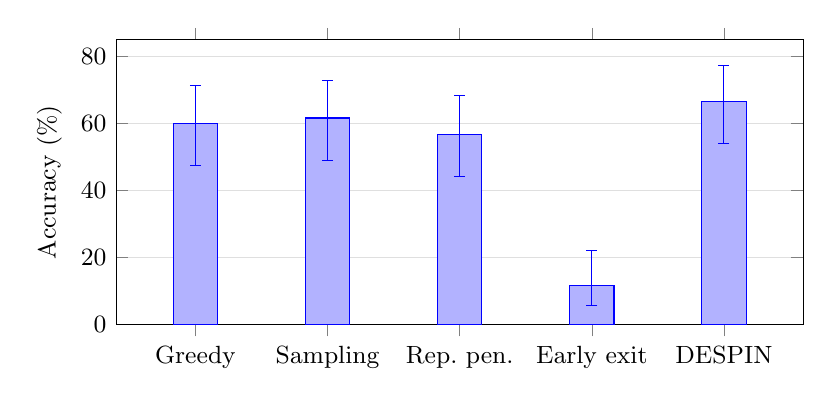
\begin{tikzpicture}
\begin{axis}[ybar, width=0.85\textwidth, height=5.2cm, ymin=0, ymax=85, ylabel={Accuracy (\%)},
  xtick={0,1,2,3,4}, xticklabels={Greedy, Sampling, Rep.\ pen., Early exit, DESPIN},
  bar width=16pt, enlarge x limits=0.15, ymajorgrids, grid style={gray!25},
  tick label style={font=\small}, label style={font=\small}]
% AUTO-GENERATED
\addplot+[ybar, error bars/.cd, y dir=both, y explicit] coordinates {
(0,60.00) += (0,11.43) -= (0,12.63)
(1,61.67) += (0,11.25) -= (0,12.65)
(2,56.67) += (0,11.76) -= (0,12.56)
(3,11.67) += (0,10.51) -= (0,5.90)
(4,66.67) += (0,10.60) -= (0,12.61)
};

\end{axis}
\end{tikzpicture}
\caption{Overall accuracy with 95\% Wilson intervals ($n=60$). The intervals for greedy decoding, sampling, repetition penalty and DESPIN overlap almost completely.}
\label{fig:acc}
\end{figure}

DESPIN reaches \statDespinCorrect/60 (\statDespinAcc\%) against \statGreedyCorrect/60 (\statGreedyAcc\%) for greedy decoding. All of the gain is on MATH (\statDespinMathCorrect/30 against \statGreedyMathCorrect/30); GSM8K is unchanged at \statDespinGsmCorrect/30. Only DESPIN solves \statNDespinVsGreedyOnlyMethod{} problems and only greedy decoding solves \statNDespinVsGreedyOnlyGreedy{} (exact $p=\statPDespinVsGreedy$). Against sampling the split is \statNDespinVsSamplingOnlyDespin{} to \statNDespinVsSamplingOnlyOther{} ($p=\statPDespinVsSampling$), and against repetition penalty it is \statNDespinVsRepetitionPenaltyOnlyDespin{} to \statNDespinVsRepetitionPenaltyOnlyOther{} ($p=\statPDespinVsRepetitionPenalty$). Sampling and greedy decoding themselves split \statNSamplingVsGreedyOnlyMethod{} to \statNSamplingVsGreedyOnlyGreedy{} on the problems where they disagree, so a difference of four problems is about what a different decoding seed can produce. The only baseline that is clearly separable from greedy decoding is early exit, and it is separable in the wrong direction.

\subsection{Where the gains come from}

\begin{table}[t]
\centering
\caption{The \statRescueCount{} problems solved by DESPIN but not by greedy decoding (from the logged records). ``Re-dec.'' is the number of discarded tokens. ``Len.\ G / D'' is the kept length under greedy decoding and under DESPIN, and ``End'' is how the DESPIN run ended (token cap or end-of-sequence). Triggers are given as type (R recurrence, V velocity collapse) and trigger position $\to$ rewind position.}
\label{tab:rescues}
\footnotesize
\setlength{\tabcolsep}{3pt}
\begin{tabular}{llccclc}
\toprule
Problem & Subject (level) & Len.\ G / D & Re-dec. & End & Triggers & Answer \\
\midrule
math500\_1 & Int.\ Algebra (5) & 2048 / 2048 & 143 & cap & R $166\!\to\!54$; V $104\!\to\!73$ & \texttt{p-q} \\
math500\_10 & Number Theory (3) & 2048 / 2048 & 95 & cap & V $124\!\to\!68$; V $135\!\to\!96$ & \texttt{2220} \\
math500\_26 & Count.\ \& Prob.\ (5) & 2048 / 2048 & 112 & cap & R $290\!\to\!219$; V $510\!\to\!469$ & \texttt{144} \\
math500\_28 & Precalculus (2) & 2048 / 1798 & 53 & EOS & V $174\!\to\!138$; V $182\!\to\!165$ & \texttt{-2+7i} \\
\bottomrule
\end{tabular}
\end{table}

Table~\ref{tab:rescues} lists the four gains. Only \texttt{math500\_28} ended with an end-of-sequence token. The other three stopped at the cap, so there is no finished final response, and the scored string came either from a \texttt{\textbackslash boxed} expression inside the reasoning or from the fallback extractor; since the texts were not stored, the logs cannot tell which. Across the \statDespinCappedN{} DESPIN runs that hit the cap, \statPrunedInCappedDespin{} tokens were re-decoded, which is extra decoding compared with a baseline whose cap covers everything it decodes. Greedy decoding hit the cap on \statGreedyCapHits{} of the 30 MATH problems, and \statGreedyCorrectCapped{} of its \statGreedyCorrect{} correct answers are capped runs, so on this problem set accuracy is largely a measure of behavior under truncation.

\subsection{Token cost}\label{sec:compute}

The earlier draft reported an average length of $1{,}120.5$ tokens for DESPIN against $1{,}148.5$ for greedy decoding, and a token efficiency score (TES) of $59.50$ against $52.24$. Those lengths leave out \statPrunedTotal{} discarded tokens, \statPrunedMean{} per problem. With them included, DESPIN decodes \statDespinAvgTotal{} tokens per problem, which is \statTotalRatio\% relative to greedy decoding (the kept length alone is \statFinalRatio\%), and its TES drops from \statDespinTESFinal{} to \statDespinTESTotal{}. Per correct answer DESPIN uses \statDespinTokPerCorrect{} tokens against \statGreedyTokPerCorrect{} for greedy decoding, a \statTokPerCorrectGain\% reduction, but that figure rests on the same four gains. TES is also not a good summary here: the early-exit baseline scores \statEarlyTESFinal{}, close to greedy's \statGreedyTESFinal{}, while solving only \statEarlyCorrect{} of 60 problems.

\subsection{How selective the detector is}

\begin{figure}[t]
\centering
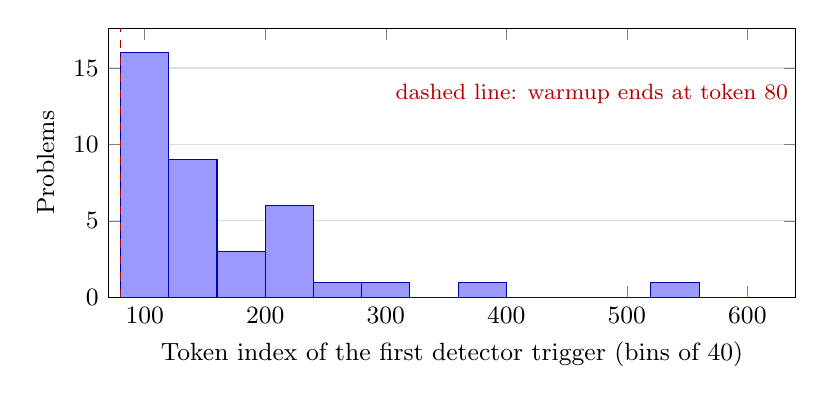
\begin{tikzpicture}
\begin{axis}[width=0.85\textwidth, height=5cm, xlabel={Token index of the first detector trigger (bins of 40)}, ylabel={Problems},
  xmin=70, xmax=640, ymin=0, ymajorgrids, grid style={gray!25}, tick label style={font=\small}, label style={font=\small}]
% AUTO-GENERATED
\addplot+[ybar interval, fill=blue!40, draw=blue!70!black, mark=none] coordinates {
(80,16) (120,9) (160,3) (200,6) (240,1) (280,1) (320,0) (360,1) (400,0) (440,0) (480,0) (520,1) (560,0) (600,0)
};

\draw[red!70!black, dashed] (axis cs:80,0) -- (axis cs:80,\pgfkeysvalueof{/pgfplots/ymax});
\node[red!70!black, font=\footnotesize, anchor=south west] at (axis cs:300,12) {dashed line: warmup ends at token 80};
\end{axis}
\end{tikzpicture}
\caption{Position of the first detector trigger in the \statFirstTrigN{} problems where DESPIN fired (median \statFirstTrigMedian, mean \statFirstTrigMean{} tokens). \statFirstTrigEarly{} of \statFirstTrigN{} trigger within 220 tokens.}
\label{fig:trigger}
\end{figure}

The detector fires on \statTrigAny{} of the 60 problems: \statTrigMath{} of 30 MATH and \statTrigGsm{} of 30 GSM8K. Greedy decoding hit the cap on \statGreedyCappedN{} problems, and the detector fired on \statGreedyCappedTrig{} of them. It also fired on \statHealthyTrig{} of the \statHealthyN{} problems that greedy decoding solved and finished before the cap. The first firing is usually the first eligible boundary after the warmup (Figure~\ref{fig:trigger}); of the \statFirstTrigN{} first triggers, \statVelFirst{} are velocity collapses and \statRecFirst{} are recurrences. So the detector does react to the loops in the capped runs, but it reacts to most other runs as well. That is plausible for post-norm final-layer states, whose consecutive step states are strongly aligned in many decoders, but we did not measure the baseline cosine distribution, so we cannot make that statement quantitative.

The early-exit baseline shows what this means in practice. Because it stops at the first firing, it truncated \statEarlyTruncated{} of 60 generations, at a median of \statEarlyMedianLen{} tokens (maximum \statEarlyMaxLen). Its accuracy of \statEarlyAcc\% describes this detector's firing rate. It is not evidence that loop detection alone is insufficient, which is what the earlier draft concluded from it. Two of its \statEarlyCorrect{} correct answers (math500\_12 and gsm8k\_20) are truncated runs where the gold answer also appears in the problem statement, which fits the fallback extractor picking up a number copied from the question.

\subsection{What the rollbacks actually do}

\begin{figure}[t]
\centering
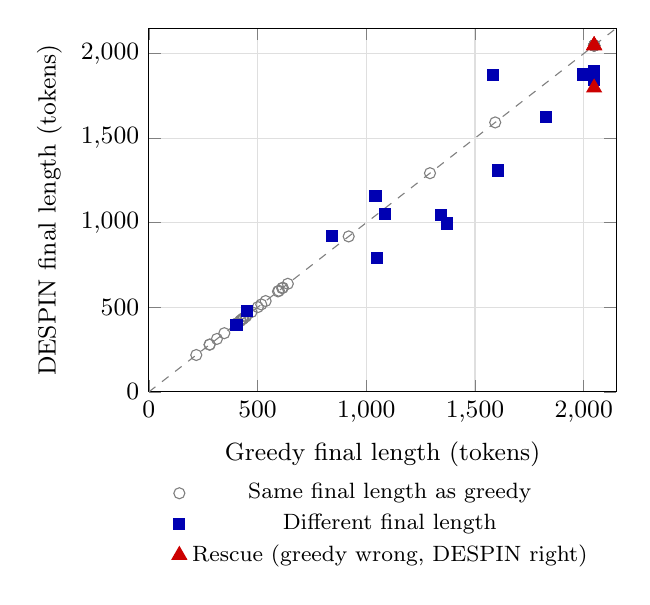
\begin{tikzpicture}
\begin{axis}[width=0.62\textwidth, height=6.2cm, xlabel={Greedy final length (tokens)}, ylabel={DESPIN final length (tokens)},
  xmin=0, xmax=2150, ymin=0, ymax=2150, legend style={font=\footnotesize, draw=none, at={(0.5,-0.22)}, anchor=north}, xtick={0,500,1000,1500,2000},
  ymajorgrids, xmajorgrids, grid style={gray!25}, tick label style={font=\small}, label style={font=\small}]
\addplot[domain=0:2150, gray, dashed, forget plot] {x};
% AUTO-GENERATED
\addplot[only marks, mark=o, color=gray] coordinates {(1293,1293) (1593,1593) (2048,2048) (919,919) (2048,2048) (2048,2048) (2048,2048) (2048,2048) (347,347) (2048,2048) (2048,2048) (2048,2048) (2048,2048) (2048,2048) (2048,2048) (2048,2048) (2048,2048) (448,448) (279,279) (517,517) (218,218) (421,421) (280,280) (423,423) (639,639) (616,616) (404,404) (404,404) (472,472) (421,421) (613,613) (401,401) (594,594) (537,537) (430,430) (598,598) (444,444) (405,405) (435,435) (501,501) (313,313) (433,433)};
\addlegendentry{Same final length as greedy}
\addplot[only marks, mark=square*, color=blue!70!black] coordinates {(844,921) (1995,1876) (1343,1046) (2048,1846) (1050,792) (1583,1873) (2048,1895) (1042,1156) (1827,1623) (1606,1309) (1087,1053) (1370,996) (450,480) (403,397)};
\addlegendentry{Different final length}
\addplot[only marks, mark=triangle*, color=red!80!black, mark size=3pt] coordinates {(2048,2048) (2048,2048) (2048,2048) (2048,1798)};
\addlegendentry{Rescue (greedy wrong, DESPIN right)}

\end{axis}
\end{tikzpicture}
\caption{Final length under greedy decoding against DESPIN, one point per problem. Points on the diagonal are runs where the controller left the kept length unchanged.}
\label{fig:scatter}
\end{figure}

DESPIN executed at least one rollback on \statAsdProblems{} problems, and on \statAsdAtCap{} of them it used both rollbacks it was allowed. The final length differs from greedy decoding on only \statLenChanged{} of 60 problems (Figure~\ref{fig:scatter}), and all of those have a trigger. Two things suggest that many rollbacks do nothing. First, on \statNoopCount{} problems that ended before the cap (math500\_2, 3 and 5; gsm8k\_13, 15, 24 and 26) the final length with rollbacks is exactly the greedy length, which is what we would expect if the regenerated text is identical. Second, on \statDupProblems{} problems the two logged rollback events are identical in trigger position, rewind position and similarity. That means the model walked back into the same trajectory after the first rollback, and the penalty of Eq.~\eqref{eq:asd} did not change a single argmax; \statDupWasted{} of the \statPrunedTotal{} discarded tokens come from these cases. Without stored texts, identical length is evidence of identical output, not proof. Early closure fired \statPgecN{} times, always on a correct answer. It shortened the run \statPgecShorter{} times and lengthened it in the others (mean change $-\statPgecMeanDelta$ tokens), because the closures happen after earlier rollbacks have already changed the trajectory.

\subsection{Scoring problems}

Three things about the extractor and normalizer matter. First, the normalization strips every comma and closing brace and does not treat \texttt{\textbackslash dfrac} as \texttt{\textbackslash frac}. The answer to math500\_0 (polar coordinates $(3,\pi/2)$) is therefore scored wrong for every method, even though DESPIN's logged string \texttt{\textbackslash left(3,\allowbreak\textbackslash dfrac\{\allowbreak\textbackslash pi\{2\allowbreak\textbackslash right)} is the correct answer. Second, a percentage is not matched to a bare number: gsm8k\_14 (gold 60) is scored wrong for an answer of \texttt{60\%}. DESPIN's logged answers to both problems are correct, so a corrected scorer would raise DESPIN to $42/60$. Greedy decoding's extracted strings for the final run were not stored (on gsm8k\_14 it has the same kept length as DESPIN and no trigger, so it presumably gave the same answer), so the effect on the paired difference cannot be established from the logs. Third, the fallback heuristics were extended with strings taken from this benchmark's own outputs, for example \texttt{thedoublesumisp-q}, which is the DESPIN output for math500\_1. In other words the scorer was adjusted after seeing results. A corrected evaluator with unit tests is released; the numbers above use the original one.

\subsection{The boundary, and where the simple story breaks}\label{sec:boundary}

Table~\ref{tab:corrections} lists every claim of the earlier draft that the logs or the code do not support. Each was checked against \texttt{data/logged\_run/} or against the scripts, and none of them needs a new experiment to settle.

\begin{table}[t]
\centering
\caption{Claims in the earlier draft that are withdrawn or corrected.}
\label{tab:corrections}
\footnotesize
\begin{tabularx}{\textwidth}{>{\raggedright\arraybackslash}p{4.3cm}X}
\toprule
Earlier claim & What the logs and code show \\
\midrule
Rescued \texttt{math500\_1}, \texttt{\_8}, \texttt{\_13}, \texttt{\_22} & The rescued problems are \texttt{math500\_1, \_10, \_26, \_28}. Greedy decoding already solved \texttt{\_8} and \texttt{\_13}, and \texttt{\_22} fails under every method. \\
Case study: $107n\equiv27 \pmod{1000}$, rollback of 74 tokens to token 212, 1{,}152 tokens, $\boxed{27}$ & \texttt{math500\_1} is the $p=\sum 1/k^2$, $q=\sum1/k^3$ problem (gold $p-q$). The logged rollbacks are $166\to54$ and $104\to73$, and the run used 2{,}048 tokens. The case study matches no logged run and is removed. \\
``Zero false rollbacks'' on GSM8K & \statTrigGsm{} GSM8K problems triggered the controller. Greedy decoding solved all of them too. \\
``Strictly dominates all baselines'' & Early exit uses fewer tokens, sampling solves more GSM8K problems (24 against 22), and DESPIN is not significantly different from any baseline except early exit. \\
``Reduces token consumption'' & Kept length $\statFinalRatio\%$, total decoded tokens $\statTotalRatio\%$ compared with greedy. \\
``Stratified across 7 disciplines'' & The first 30 items in dataset order; the counts differ from the earlier appendix table (Section~\ref{sec:setup}). The earlier remark about failed Level-5 Geometry items is unsupported, because the set has no Level-5 Geometry item. \\
Thresholds ``calibrated on pilot traces'' & The calibration script uses two traces, \texttt{gsm8k\_0} and \texttt{math500\_1}, both inside the evaluation set, and several engine variants were iterated on \texttt{math500\_1}. \\
Early exit is \citet{wei2025stop} & It is the same detector stopping generation, not their method. \\
Recurrence heatmap of a ``looping'' trace & The ``loop'' panel was \texttt{gsm8k\_0} cut off at 400 tokens, a problem that greedy decoding solves in 448 tokens without any loop, and the ``healthy'' panel was a different problem. It is not a rollout from the benchmark and is removed. \\
Case-study schematic (1{,}024 against 478 tokens, answer 24) & The text was hard-coded in the plotting script. The logged run of \texttt{gsm8k\_0} used 448 tokens, was correct, and had no rollback. Removed. \\
Latency breakdown (forward step, cosine scan, projection) & Only KV-crop times are logged (0.13 to 0.21\,ms). No script in the repository measures the other components, so they are removed. Greedy/DESPIN and the other baselines were timed in two separate runs whose per-token speeds differ a lot, so latencies are not comparable and are not reported. \\
Seeds fixed; greedy checked against \texttt{generate}; KV tensor-hash checks & No seed is set in the sweep scripts and no script performs these checks, so we do not claim them. \\
Theorem~1 establishes the method & The identity is plain linearity and does not describe Eq.~\eqref{eq:asd} (Section~\ref{sec:rollback}). \\
References & Three entries had wrong authors or identifiers (circular reasoning, backtracking bursts, LoopGuard) and one could not be verified. All were replaced or dropped (Appendix~\ref{app:refs}). \\
\bottomrule
\end{tabularx}
\end{table}

\section{Discussion}

What the logs support is a narrow statement: on 60 problems and one run per method, DESPIN solved four more problems than greedy decoding and lost none. They do not support a claim of improvement over sampling or repetition penalty, a token saving, an ability to diagnose loops, or any special role for the deflation step.

Three other explanations for the four gains are still open. One is rollback as a restart: any perturbation around token 130 gives a long run a second chance, and sampling would do the same. The \statNSamplingVsGreedyOnlyMethod{} to \statNSamplingVsGreedyOnlyGreedy{} split between sampling and greedy decoding shows how large such differences are at this sample size. Another is budget: the kept-length cap gave DESPIN extra decoding in the capped runs. The third is scoring: \statRescueCapped{} of the gains were judged on unfinished text.

The released script \texttt{scripts/run\_controls.py} is meant to separate these explanations. It runs rollback with the deflation switched off (C1), rollback with a random unit direction in place of $u$ (C2), DESPIN with the 2{,}048-token cap applied to all decoded tokens (C3), sampling with several seeds (C4), and early closure alone (C5), and it stores the full generated text of every run. A threshold sweep calibrated on items that are not in the evaluation set, and a run on the full 500-problem MATH-500 set and on GSM8K, would be needed for real statistical power. None of this has been run yet, and this paper reports no new generations.

\paragraph{Limitations.} Our evidence comes from one 1.5B model, one run per method and 60 problems, and $19$ of the $30$ MATH items hit the cap under greedy decoding. The generated texts were not stored, so several statements above are inferences from lengths. The sampling baseline has no seed, and the scorer has known false negatives. We report these openly rather than leaving them out, because each of them limits how much weight the four gains can carry.

\section{Conclusion}

We took a positive result about inference-time rollback for reasoning loops and re-checked it against the raw logs. The headline difference is there, but it is four net problems out of sixty, it is not significant, part of it rests on unfinished generations and extra decoding budget, and it comes from a detector that fires on most problems, including most that were already solved. Several supporting claims, a case study and two figures in the earlier draft did not match the data and are withdrawn. Whether directional deflation does anything beyond restarting the generation is still open, and the control suite released with this paper is meant to answer it.

\section*{Code and Data Availability}
{\sloppy Code, logs and the analysis script are publicly available at \url{https://github.com/Feonixid/DESPIN-Reasoning}. The logged run is in \texttt{data/\allowbreak logged\_run/}, and \texttt{python scripts/\allowbreak make\_paper\_\allowbreak assets.py} regenerates every number, table and figure-data file in this paper (\texttt{paper/\allowbreak generated/}) from it; on Windows, \texttt{run\_all.bat} does this and builds the paper. The scripts and engine versions that produced the logs are kept in \texttt{legacy/\allowbreak logged\_run/}.\par}

\appendix

\section{Hyperparameters of the logged run}\label{app:hparams}
\begin{center}
\small
\begin{tabular}{ll}
\toprule
Parameter & Value \\
\midrule
Recurrence threshold $\tau_{\rm recur}$ & 0.90 \\
Velocity threshold $\tau_v$, consecutive boundaries & 0.18, 2 \\
Minimum step length $L_{\min}$ & 6 tokens \\
Warmup & 80 tokens \\
Deflation $\gamma$, window $E$ & 15, 6 tokens (linear decay) \\
Maximum rollbacks per generation & 2 \\
Maximum new tokens & 2{,}048 \\
Sampling baseline & $T=0.6$, no top-$p$, no seed \\
Repetition penalty & 1.15 (generated tokens) \\
\bottomrule
\end{tabular}
\end{center}

\section{Per-problem results}\label{app:perproblem}
Each cell shows correctness (\ding{51}/\ding{55}) and the kept length. ``Ev'' is the number of rollbacks, \texttt{+P} marks an early closure, and \texttt{*} marks two identical logged rollback events. ``Pruned'' is the number of re-decoded tokens.

% AUTO-GENERATED
{\footnotesize
\setlength{\tabcolsep}{3pt}
\begin{longtable}{llcccccccc}
\toprule
Problem & Subject & L & Greedy & Sampl. & Rep.\ pen. & Early & DESPIN & Pruned & Ev \\
\midrule
\endhead
math500\_0 & Precalculus & 2 & \ding{55} 844 & \ding{55} 1857 & \ding{55} 1379 & \ding{55} 108 & \ding{55} 921 & 63 & 2 \\
math500\_1 & Int. Algebra & 5 & \ding{55} 2048 & \ding{55} 2048 & \ding{55} 2048 & \ding{55} 166 & \ding{51} 2048 & 143 & 2 \\
math500\_2 & Algebra & 3 & \ding{51} 1293 & \ding{51} 1781 & \ding{51} 1529 & \ding{55} 107 & \ding{51} 1293 & 63 & 2 \\
math500\_3 & Number Theory & 3 & \ding{51} 1593 & \ding{51} 1167 & \ding{51} 2048 & \ding{55} 98 & \ding{51} 1593 & 81 & 2 \\
math500\_4 & Algebra & 2 & \ding{55} 2048 & \ding{55} 2048 & \ding{55} 2048 & \ding{55} 93 & \ding{55} 2048 & 95 & 2 \\
math500\_5 & Prealgebra & 2 & \ding{51} 919 & \ding{51} 899 & \ding{51} 1376 & \ding{55} 202 & \ding{51} 919 & 200 & 2* \\
math500\_6 & Number Theory & 3 & \ding{51} 1995 & \ding{51} 2048 & \ding{55} 2048 & \ding{55} 109 & \ding{51} 1876 & 91 & 2+P \\
math500\_7 & Precalculus & 4 & \ding{51} 2048 & \ding{51} 2048 & \ding{51} 2048 & \ding{55} 140 & \ding{51} 2048 & 72 & 2 \\
math500\_8 & Algebra & 3 & \ding{51} 1343 & \ding{51} 1560 & \ding{51} 1894 & \ding{55} 118 & \ding{51} 1046 & 81 & 2+P \\
math500\_9 & Prealgebra & 5 & \ding{55} 2048 & \ding{55} 2048 & \ding{55} 2048 & \ding{55} 104 & \ding{55} 2048 & 104 & 2 \\
math500\_10 & Number Theory & 3 & \ding{55} 2048 & \ding{55} 2048 & \ding{55} 2048 & \ding{55} 124 & \ding{51} 2048 & 95 & 2 \\
math500\_11 & Int. Algebra & 5 & \ding{55} 2048 & \ding{55} 2048 & \ding{55} 2048 & \ding{55} 214 & \ding{55} 2048 & 96 & 2 \\
math500\_12 & Number Theory & 5 & \ding{51} 2048 & \ding{51} 2048 & \ding{51} 2048 & \ding{51} 153 & \ding{51} 2048 & 156 & 2* \\
math500\_13 & Geometry & 2 & \ding{51} 347 & \ding{51} 460 & \ding{51} 335 & \ding{51} 281 & \ding{51} 347 & 0 & 0 \\
math500\_14 & Precalculus & 1 & \ding{55} 2048 & \ding{51} 1702 & \ding{51} 1908 & \ding{55} 118 & \ding{55} 2048 & 81 & 2 \\
math500\_15 & Precalculus & 5 & \ding{55} 2048 & \ding{55} 2048 & \ding{55} 2048 & \ding{55} 541 & \ding{55} 2048 & 586 & 2* \\
math500\_16 & Int. Algebra & 1 & \ding{51} 2048 & \ding{55} 2048 & \ding{51} 2048 & \ding{55} 107 & \ding{51} 1846 & 96 & 2+P \\
math500\_17 & Precalculus & 4 & \ding{55} 2048 & \ding{55} 2048 & \ding{55} 2048 & \ding{55} 218 & \ding{55} 2048 & 131 & 2 \\
math500\_18 & Geometry & 1 & \ding{55} 2048 & \ding{55} 2048 & \ding{55} 2048 & \ding{55} 113 & \ding{55} 2048 & 172 & 2* \\
math500\_19 & Int. Algebra & 3 & \ding{55} 2048 & \ding{55} 2048 & \ding{51} 2048 & \ding{55} 115 & \ding{55} 2048 & 41 & 2 \\
math500\_20 & Algebra & 3 & \ding{51} 1050 & \ding{51} 1137 & \ding{51} 1141 & \ding{55} 119 & \ding{51} 792 & 65 & 2 \\
math500\_21 & Int. Algebra & 3 & \ding{55} 2048 & \ding{55} 2048 & \ding{55} 2048 & \ding{55} 274 & \ding{55} 2048 & 63 & 2 \\
math500\_22 & Algebra & 5 & \ding{55} 2048 & \ding{55} 2048 & \ding{55} 2048 & \ding{55} 127 & \ding{55} 2048 & 154 & 2 \\
math500\_23 & Algebra & 5 & \ding{51} 1583 & \ding{51} 1594 & \ding{51} 1946 & \ding{55} 179 & \ding{51} 1873 & 40 & 2+P \\
math500\_24 & Algebra & 5 & \ding{51} 2048 & \ding{55} 2048 & \ding{55} 2048 & \ding{55} 217 & \ding{51} 1895 & 122 & 2+P \\
math500\_25 & Int. Algebra & 5 & \ding{55} 2048 & \ding{55} 2048 & \ding{55} 2048 & \ding{55} 133 & \ding{55} 2048 & 126 & 2* \\
math500\_26 & Count. \& Prob. & 5 & \ding{55} 2048 & \ding{55} 2048 & \ding{55} 2048 & \ding{55} 290 & \ding{51} 2048 & 112 & 2 \\
math500\_27 & Prealgebra & 2 & \ding{51} 1042 & \ding{51} 1068 & \ding{51} 1399 & \ding{55} 128 & \ding{51} 1156 & 55 & 2+P \\
math500\_28 & Precalculus & 2 & \ding{55} 2048 & \ding{55} 2048 & \ding{51} 2048 & \ding{55} 174 & \ding{51} 1798 & 53 & 2 \\
math500\_29 & Count. \& Prob. & 2 & \ding{51} 1827 & \ding{51} 1436 & \ding{51} 1325 & \ding{55} 112 & \ding{51} 1623 & 81 & 2 \\
gsm8k\_0 & Arithmetic & -- & \ding{51} 448 & \ding{51} 353 & \ding{51} 369 & \ding{55} 350 & \ding{51} 448 & 0 & 0 \\
gsm8k\_1 & Arithmetic & -- & \ding{51} 279 & \ding{51} 268 & \ding{51} 292 & \ding{51} 279 & \ding{51} 279 & 0 & 0 \\
gsm8k\_2 & Arithmetic & -- & \ding{55} 517 & \ding{55} 548 & \ding{55} 534 & \ding{55} 453 & \ding{55} 517 & 0 & 0 \\
gsm8k\_3 & Arithmetic & -- & \ding{55} 218 & \ding{55} 199 & \ding{55} 206 & \ding{55} 218 & \ding{55} 218 & 0 & 0 \\
gsm8k\_4 & Arithmetic & -- & \ding{51} 421 & \ding{51} 419 & \ding{55} 468 & \ding{55} 402 & \ding{51} 421 & 0 & 0 \\
gsm8k\_5 & Arithmetic & -- & \ding{51} 280 & \ding{51} 303 & \ding{51} 381 & \ding{51} 280 & \ding{51} 280 & 0 & 0 \\
gsm8k\_6 & Arithmetic & -- & \ding{51} 423 & \ding{51} 415 & \ding{51} 323 & \ding{51} 403 & \ding{51} 423 & 0 & 0 \\
gsm8k\_7 & Arithmetic & -- & \ding{55} 639 & \ding{55} 634 & \ding{55} 1436 & \ding{55} 494 & \ding{55} 639 & 0 & 0 \\
gsm8k\_8 & Arithmetic & -- & \ding{55} 616 & \ding{51} 2048 & \ding{55} 839 & \ding{55} 598 & \ding{55} 616 & 0 & 0 \\
gsm8k\_9 & Arithmetic & -- & \ding{51} 404 & \ding{51} 441 & \ding{51} 523 & \ding{55} 183 & \ding{51} 404 & 0 & 0 \\
gsm8k\_10 & Arithmetic & -- & \ding{51} 404 & \ding{51} 385 & \ding{51} 486 & \ding{55} 265 & \ding{51} 404 & 0 & 0 \\
gsm8k\_11 & Arithmetic & -- & \ding{51} 472 & \ding{51} 391 & \ding{51} 436 & \ding{55} 351 & \ding{51} 472 & 0 & 0 \\
gsm8k\_12 & Arithmetic & -- & \ding{55} 421 & \ding{55} 637 & \ding{55} 510 & \ding{55} 361 & \ding{55} 421 & 0 & 0 \\
gsm8k\_13 & Arithmetic & -- & \ding{51} 613 & \ding{51} 635 & \ding{51} 588 & \ding{55} 235 & \ding{51} 613 & 37 & 1 \\
gsm8k\_14 & Arithmetic & -- & \ding{55} 401 & \ding{55} 1049 & \ding{55} 425 & \ding{55} 296 & \ding{55} 401 & 0 & 0 \\
gsm8k\_15 & Arithmetic & -- & \ding{51} 594 & \ding{51} 669 & \ding{55} 507 & \ding{55} 200 & \ding{51} 594 & 168 & 2* \\
gsm8k\_16 & Arithmetic & -- & \ding{51} 1606 & \ding{51} 798 & \ding{51} 811 & \ding{55} 141 & \ding{51} 1309 & 70 & 2 \\
gsm8k\_17 & Arithmetic & -- & \ding{51} 537 & \ding{51} 419 & \ding{51} 447 & \ding{55} 519 & \ding{51} 537 & 0 & 0 \\
gsm8k\_18 & Arithmetic & -- & \ding{51} 430 & \ding{51} 383 & \ding{51} 380 & \ding{55} 290 & \ding{51} 430 & 0 & 0 \\
gsm8k\_19 & Arithmetic & -- & \ding{51} 1087 & \ding{51} 2048 & \ding{51} 1325 & \ding{55} 120 & \ding{51} 1053 & 121 & 2+P \\
gsm8k\_20 & Arithmetic & -- & \ding{55} 598 & \ding{51} 753 & \ding{51} 599 & \ding{51} 324 & \ding{55} 598 & 0 & 0 \\
gsm8k\_21 & Arithmetic & -- & \ding{55} 444 & \ding{55} 325 & \ding{55} 485 & \ding{55} 288 & \ding{55} 444 & 0 & 0 \\
gsm8k\_22 & Arithmetic & -- & \ding{51} 405 & \ding{51} 423 & \ding{51} 390 & \ding{55} 284 & \ding{51} 405 & 0 & 0 \\
gsm8k\_23 & Arithmetic & -- & \ding{51} 1370 & \ding{51} 1067 & \ding{55} 1162 & \ding{55} 113 & \ding{51} 996 & 65 & 2 \\
gsm8k\_24 & Arithmetic & -- & \ding{51} 435 & \ding{51} 415 & \ding{51} 388 & \ding{55} 100 & \ding{51} 435 & 156 & 2* \\
gsm8k\_25 & Arithmetic & -- & \ding{51} 450 & \ding{51} 418 & \ding{51} 555 & \ding{55} 150 & \ding{51} 480 & 44 & 1 \\
gsm8k\_26 & Arithmetic & -- & \ding{51} 501 & \ding{51} 469 & \ding{51} 474 & \ding{55} 91 & \ding{51} 501 & 130 & 2* \\
gsm8k\_27 & Arithmetic & -- & \ding{51} 403 & \ding{51} 437 & \ding{51} 458 & \ding{55} 308 & \ding{51} 397 & 0 & 0+P \\
gsm8k\_28 & Arithmetic & -- & \ding{51} 313 & \ding{51} 375 & \ding{55} 476 & \ding{51} 313 & \ding{51} 313 & 0 & 0 \\
gsm8k\_29 & Arithmetic & -- & \ding{51} 433 & \ding{51} 399 & \ding{51} 463 & \ding{55} 335 & \ding{51} 433 & 0 & 0 \\
\bottomrule
\end{longtable}
}


\section{Reference audit}\label{app:refs}
The earlier bibliography credited ``Circular Reasoning'' to authors who did not write it, with arXiv identifier 2601.08942. The paper is arXiv:2601.05693 by Duan et al., and it proposes a CUSUM detector on hidden states, not the PCA-trajectory analysis described in the earlier text. ``The Shape of Overthinking'' is by Rezazadeh and Davoodi (arXiv:2605.27965). LoopGuard is arXiv:2604.10044 by Xu et al. and targets repetition in long-context generation under a fixed cache budget. The reasoning completion point belongs to \citet{wei2025stop}, not to the entry that was attributed to Google DeepMind, which we could not verify and dropped. The five 2025 and 2026 entries that matter for this work (Duan et al., Wei et al., Huang et al., Xu et al., Rezazadeh and Davoodi) were checked against arXiv or proceedings pages on November 7, 2026. The remaining entries (datasets, classical references, the library citation) were not re-checked and should be verified before submission.

\begin{thebibliography}{14}\small
\setlength{\itemsep}{0.45em}

\bibitem[Snell et al.(2024)]{snell2024scaling}
Snell, C., Lee, J., Xu, K., and Kumar, A.
Scaling LLM test-time compute optimally can be more effective than scaling model parameters.
\emph{arXiv preprint arXiv:2408.03314}, 2024.

\bibitem[DeepSeek-AI(2025)]{deepseek2025r1}
DeepSeek-AI.
DeepSeek-R1: Incentivizing reasoning capability in LLMs via reinforcement learning.
\emph{arXiv preprint arXiv:2501.12948}, 2025.

\bibitem[Duan et al.(2026)]{duan2026circular}
Duan, Z., Pang, L., Wei, Z., Duan, W., Tian, Y., Xu, S., Deng, J., Yin, Z., and Cheng, X.
Circular reasoning: Understanding self-reinforcing loops in large reasoning models.
\emph{arXiv preprint arXiv:2601.05693}, 2026.

\bibitem[Wei et al.(2025)]{wei2025stop}
Wei, Z., Pang, L., Liu, J., Deng, J., Xu, S., Duan, Z., Wang, J., Sun, F., Cai, X., Shen, H., and Cheng, X.
Stop spinning wheels: Mitigating LLM overthinking via mining patterns for early reasoning exit.
\emph{arXiv preprint arXiv:2508.17627}, 2025.

\bibitem[Keskar et al.(2019)]{keskar2019ctrl}
Keskar, N. S., McCann, B., Varshney, L. R., Xiong, C., and Socher, R.
CTRL: A conditional transformer language model for controllable generation.
\emph{arXiv preprint arXiv:1909.05858}, 2019.

\bibitem[Huang et al.(2025)]{huang2025manifold}
Huang, Y., Chen, H., Ruan, S., Zhang, Y., Wei, X., and Dong, Y.
Mitigating overthinking in large reasoning models via manifold steering.
In \emph{Advances in Neural Information Processing Systems}, 2025.

\bibitem[Xu et al.(2026)]{xu2026loopguard}
Xu, D., Wu, H., Shi, W., Cui, Y., Liu, Y., Li, J., Ma, H., Liu, A., Zhu, J., and Xu, J.
LoopGuard: Breaking self-reinforcing attention loops via dynamic KV cache intervention.
\emph{arXiv preprint arXiv:2604.10044}, 2026.

\bibitem[Rezazadeh and Davoodi(2026)]{rezazadeh2026shape}
Rezazadeh, N. and Davoodi, A. G.
The shape of overthinking: Backtracking bursts in long reasoning traces.
\emph{arXiv preprint arXiv:2605.27965}, 2026.

\bibitem[Wolf et al.(2020)]{wolf2020transformers}
Wolf, T., Debut, L., Sanh, V., et al.
Transformers: State-of-the-art natural language processing.
In \emph{Proceedings of the 2020 Conference on Empirical Methods in Natural Language Processing: System Demonstrations}, 2020.

\bibitem[Hendrycks et al.(2021)]{hendrycks2021math}
Hendrycks, D., Burns, C., Kadavath, S., Arora, A., Basart, S., Tang, E., Song, D., and Steinhardt, J.
Measuring mathematical problem solving with the MATH dataset.
\emph{arXiv preprint arXiv:2103.03874}, 2021.

\bibitem[Lightman et al.(2023)]{lightman2023let}
Lightman, H., Kosaraju, V., Burda, Y., et al.
Let's verify step by step.
\emph{arXiv preprint arXiv:2305.20050}, 2023.

\bibitem[Cobbe et al.(2021)]{cobbe2021gsm8k}
Cobbe, K., Kosaraju, V., Bavarian, M., et al.
Training verifiers to solve math word problems.
\emph{arXiv preprint arXiv:2110.14168}, 2021.

\bibitem[Wilson(1927)]{wilson1927probable}
Wilson, E. B.
Probable inference, the law of succession, and statistical inference.
\emph{Journal of the American Statistical Association}, 22(158):209--212, 1927.

\bibitem[McNemar(1947)]{mcnemar1947note}
McNemar, Q.
Note on the sampling error of the difference between correlated proportions or percentages.
\emph{Psychometrika}, 12(2):153--157, 1947.

\end{thebibliography}

\end{document}
